\section{Deployment}

The Processeditor consists of two components, the server which allows you to create and alter models inside your process as well as saving them to a centralized repository and the Workbench, a Rich Client which allows you to create, alter and save models locally and to publish them on a running Processeditor server.
If you want to integrate the Processeditor and the JEngine you need both components.
You can deploy them using \href{https://ant.apache.org}{Ant}\footnote{\url{https://ant.apache.org}} and Ivy.

\subsection{Cloning the Repository}

The code of the Processeditor is hosted on Github\footnote{\url{http://github.com}}.
We recommend to use git\footnote{\url{http://git-scm.com/}} to clone the repository.
To clone the repository type the following command (Figure \ref{lis:clone}):

\begin{figure}[h!]
\begin{verbatim}
	
\end{verbatim}
\caption{Command for cloning the repository using git}
\label{lis:clone}
\end{figure}

\subsection{Workbench}

The Workbench is a Rich Client for the Processeditor.
If you would like to deploy it using Ant run the following commands from the command line. Assert that you are inside the Projects root directory with the build.xml file.

\begin{figure}[h!]
\begin{verbatim}
	ant init-ivy deps clean-build-workbench
\end{verbatim}
\caption{Command for deploying the Workbench}
\label{lis:depw}
\end{figure}

Inside the build/jar folder will be a processeditor.jar file. If you execute this using java (figure \ref{lis:startworkbench}) a window with a Java application - the Workbench - will be opened.


\begin{figure}[h!]
\begin{verbatim}
	java -jar build/jar/processeditor.jar
\end{verbatim}
\caption{Command for starting the workbench}
\label{lis:startworkbench}
\end{figure}

\subsection{Server}

The server is another component of the Processeditor. It can be used as an online modeling tool and as a model repository.
If you want to deploy the server you first need to add the necessary dependencies.
All Java dependencies can be added running Ivy (figure \ref{lis:ivy}).

\begin{figure}[h!]
\begin{verbatim}
	ant init-ivy deps
\end{verbatim}
\caption{Command for downloading Java dependencies}
\label{lis:ivy}
\end{figure}

In addition you need \href{http://www.sencha.com/products/extjs/download/ext-js-4.2.1/2281}{ExtJS 4}\footnote{\url{http://www.sencha.com/products/extjs/download/ext-js-4.2.1/2281}}. This is necessary to display the components of the webmodeler. Please copy the files into \url{www/js/ext} (Figure \ref{pic:ext}).

\begin{figure}[h!]
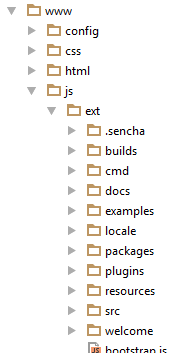
\includegraphics{graphics/wwwWithExt.png}
\caption{www folder with ExtJS dependency}
\label{pic:ext}
\end{figure}

If you have successfully completed the previous steps you can deploy the server using the command (figure \ref{lis:deps}).

\begin{figure}[h!]
\begin{verbatim}
	ant clean-build-server
\end{verbatim}
\caption{Command for deploying the Processeditor server}
\label{lis:deps}
\end{figure}

\begin{leftbar}
\textbf{
Please note:} If you need both, the Processeditor server and the Workbench, make sure to copy the jar file created during the first steps, because deploying the other component will automatically overwrite the jar.
\end{leftbar}

If you want to start the Processeditor server you can do so from the command line (figure \ref{lis:startserver}).

\begin{figure}[h!]
\begin{verbatim}
	java -jar processeditor.jar -Xmx 1024m
\end{verbatim}
\caption{Command for starting the deployed Processeditor Server}
\label{lis:startserver}
\end{figure}